
\chapter{VUV measurement}
% citare LaserLab
% perche misurare a questa energia e come
% guarda il paper di patrick

\section{High Harmonic Generation}
When an atom is exposed to a strong laser field it can absord a large number of photons through non linear processes. This energy can be transferred back to the photon field.
The phenomenon of high order harmonic generation of a laser field is a nonlinear effect that results in the emission of photons of frequency multiple of the source frequency. For example a rare gas traversed by a sufficiently power laser field may give rise to harmonic generation.
\begin{figure}[htbp]
\begin{center}
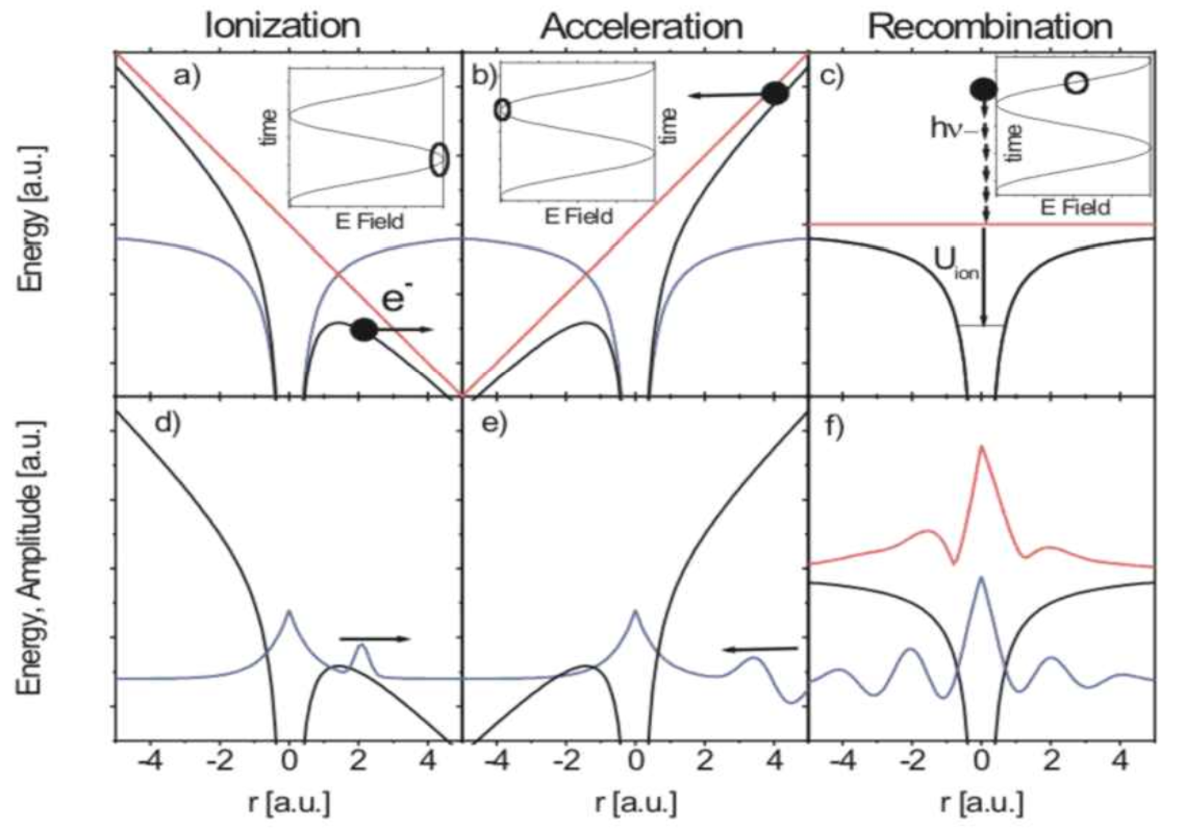
\includegraphics[width=12cm]{../Pictures/Chapter_8/HHG}
\end{center}
\caption[HHG phenomenology]{Phenomenology of High Harmonics Generation}
\label{fig:HHG}
\end{figure}

In figure \ref{fig:HHG} the main details of the high harmonic generation process are summarized, in a semi-classical configuration and as a quantum wave process.
If the laser field is strong enough ($\sim 10^{10}$V/m), it can allow the electron to tunnel through the barrier. The electron itself sits unperturbed in the well until the field of the laser sums to the atom potential bending it.
The electron gets accelerated in the laser field and it can recollide with the atom itself. The electron kinetic energy is then transferred into photons.
The cut-off energy can be calculated by examining the maximum energy the ionized electron can gain in the electric field of the laser, that is
\begin{equation}
E_{max} = I_{p}+3.17U_{p}
\end{equation}
where $U_{p}$ is the ponderomotive energy from the laser and $I_{p}$ is the ionisation potential. The recollision leads to the emission of a very broad light spectrum.
The ionization and recollision happen on each half cycle of the laser pulse, and the spectra are added coherently. As a consequence the spectrum is structured in odd harmonics.
High harmonics constitute a source of soft X-rays that retains the time characteristics of the driving laser, in terms of bunch structure and repetition rate. 
The harmonic cut off varies with the laser intensity up to saturation. The saturation intensity depends on atomic species of the noble gas used as a medium to produce the harmonics.

\section{Experimental setup}
The setup available at CELIA it is presented in \cite{Martin2001}. it will be briefly described here. The line is organized in two different room. A first room is devoted to the laser amplification system, while in the experimental room the high harmonics are produced.
\subsection{Laser beamline}
The AURORE beamline is based on a amplified Ti-sapphire femtosecond oscillator. 
The Ti-sapphire oscillator generates 30 fs pulses, at 1 nJ and a frequency of 80 MHz. Before amplification the pulses are stretched up to 280 ps for optical power reasons.
The regenerative pre amplifier brings the energy of the beam to 700 $\micro J$ at 1 kHz.
The beam is then amplified in a Ti:sapphire crystal pumped by four synchronised Nd:YLF lasers at 532 nm and 15 W.
At the end of the amplification chain the laser beam delivered has a power of 10 W for 170 ps and it is sent to the experimental room.
%figura laser
\subsection{VUV line}

\begin{figure}[htbp]
\begin{center}
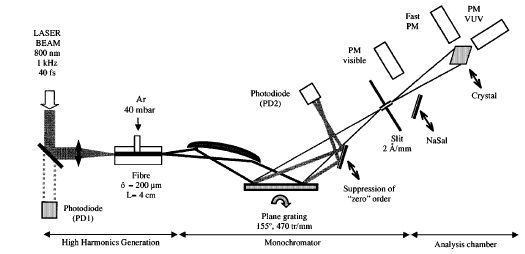
\includegraphics[width=12cm]{../Pictures/Chapter_8/VUV_line.png}
\end{center}
\caption[VUV line]{Schematics of the VUV line at CELIA Bordeaux}
\label{fig:VUV_line}
\end{figure}
Before high harmonic generation the beam is compressed again down to 35 fs, centered around 800 nm at 1 kHz, with an energy of 4 mJ.
A schematic of the HH VUV beamline is presented in fig
The elements are under vacuum at a pressure of $10^{-6}$ mbar. The beam is focused in the fiber containing the gas (200$\mi m$ in diameter and 4 cm length). Depending on the gas used and the pressure condition the energy of the harmonic lines and the efficiency of the process may vary. Tipically in Argon/Neon the energy of the harmonics is between 10 eV and 120 eV.
The fundamental beam and the harmonics spread at the exit of the fiber and are sent to the monchromator where a toroidal mirror and a plane grating (470 lines/mm) focuse the selected wavelength on the exit slit.
The zero order is suppressed by a plane mirror at an angle tuned on the grating system.
The desired VUV-XUV beam selected in energy is then directed to the sample placed in a vacuum chamber. Due to the dispersion by the grating the output pulses are stretched in time, and they have been measured with a VUV-streak camera to be 2-3 ps FWHM.
\begin{figure}[htbp]
\begin{center}
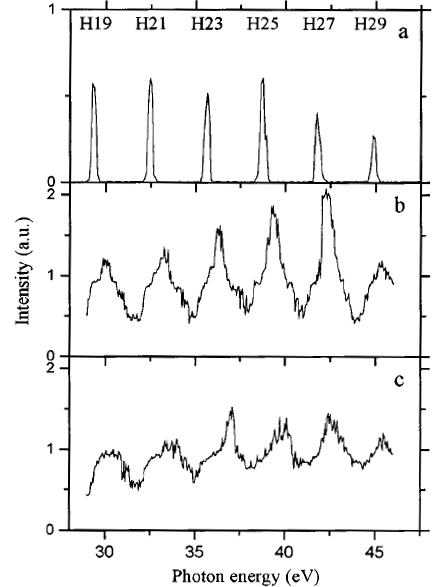
\includegraphics[width=7cm]{../Pictures/Chapter_8/VUV_spectrum.png}
\end{center}
\caption[VUV spectrum]{Schematics of the VUV line at CELIA Bordeaux}
\label{fig:VUV_spectrum}
\end{figure}
\subsection{Detection system}
The light produced by the luminescent sample hit by the VUV-XUV radiation is collected by an optical fibre visible-UV of 0.6 mm diameter mounted on a side of the chamber and connected to a monochromator (TRIAX Jobin-Yvon 130) by a focalisation system.
The monochromator is equipped with three diffraction gratings, one with 1200 lines/mm and the others with 300 lines/mm. This allows to cover a spectral range between 200 nm and 1000 nm.

%The emission spectrum is measured by mean of a CCD camera 
%manca il modello!
The photon counting device is a Hamamatsu MCP-PMT R3809U-52 model. The DAQ system is shown in figure \ref{fig:daq}.
The signal from the laser trigger is routed into a Ortec Pico Timing Discriminator (model 9307). A first output is directed directly to a Ortec Time to Analog Converter (model 9308).
A second output is directed to a Lecroy Quad Coincidence Unit (model 622).
The MCP-PMT signal is preamplified by a ORTEC 1-GHz preamplifier (model 9306) with a gain of 100 and then sent to a second Pico Timing Discriminator. One output is sent to the Lecroy Quad Coincidence Unit and a second one delayed by 60 ns and sent to the TAC. The last unit is required since the laser trigger has a fixed delay. 
A third output is sent to a SR400 Gated Photon Counter (Stanford Research System) along with the output of the Lecroy coincidence unit.
The SR400 Gated Photon Counter allows to determine the rate of counts at the MCP detector, to keep under control the fraction of biased events.
The TAC guarantees a 16-bit digital resolution in the range 0-325 $\micro$s down to a binning of 1.22 ps and its signal is sent to a computer for the software system to finally determine the delay between the MCP and the laser trigger.
\begin{figure}[htbp]
\begin{center}
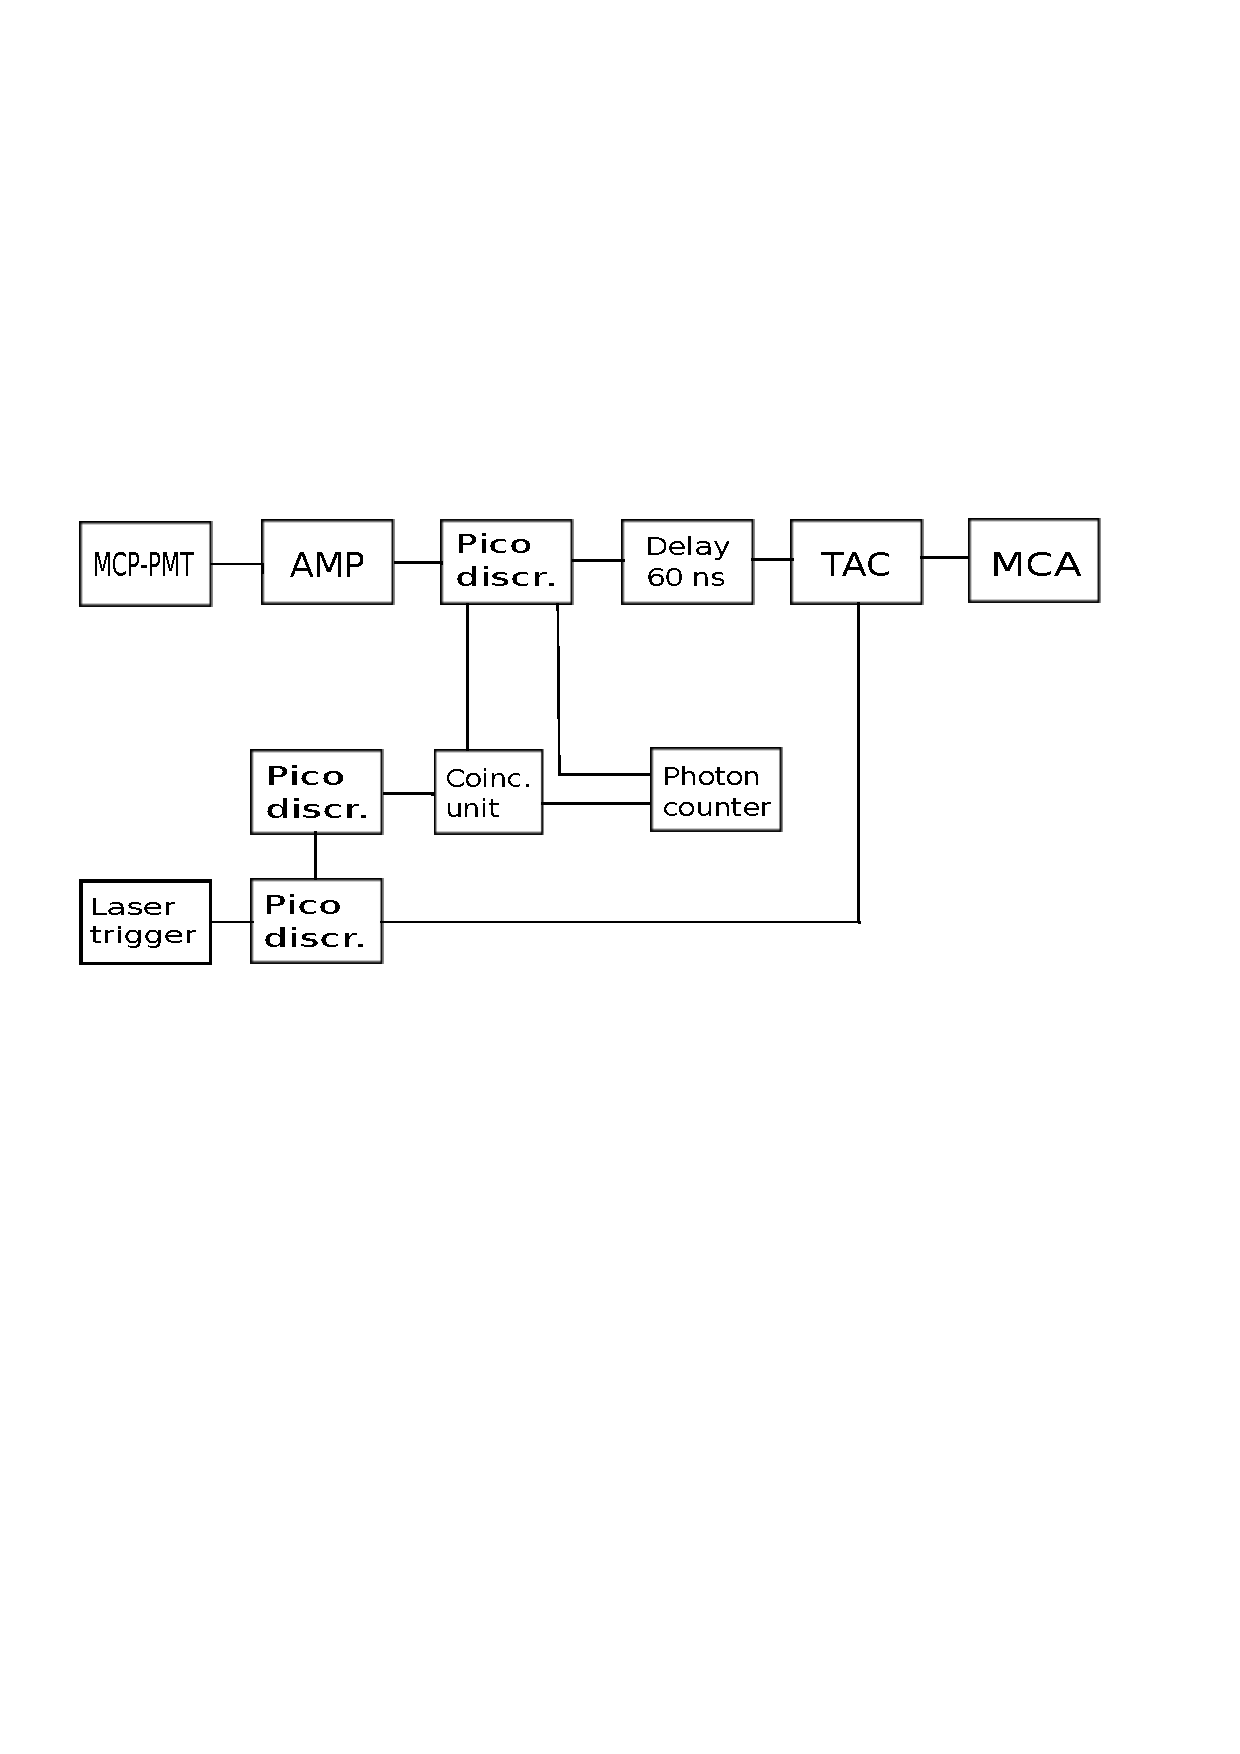
\includegraphics[width=9cm]{../Pictures/Chapter_8/electronics.pdf}
\end{center}
\caption[VUV DAQ]{Schematics of DAQ system}
\label{fig:daw}
\end{figure}

\section{Preliminaries}


\subsection{VUV spectrum}
\subsection{IRF measurement}
\subsection{Control of the bias fraction}

\section{Data analysis}
\section{Fit procedure}
\section{Results}